\chapter{Giao diện và kết quả chạy demo}
\section{Dashboard tổng quan}
Giao diện Streamlit tổ chức thành bốn tab: Hội chẩn demo, Tri thức và đồ thị, Thực nghiệm, Hướng dẫn. Phần đầu hiển thị tên hệ thống, quy mô dữ liệu, số tác tử và số ghi chú. Các nút chạy nhanh nạp đồng thời câu hỏi, hồ sơ và dữ liệu nhật ký của từng tình huống.

Trong tab hội chẩn, vùng nhập liệu gồm lựa chọn tác vụ, mô hình, câu hỏi và hồ sơ 21 chỉ báo. Hồ sơ mẫu lấy từ tập train; chế độ Nhập JSON cho phép thay toàn bộ vector đầu vào. Trạng thái của bảy tác tử được cập nhật từ thông điệp phát sinh khi chạy hệ thống.
\begin{figure}[H]\centering
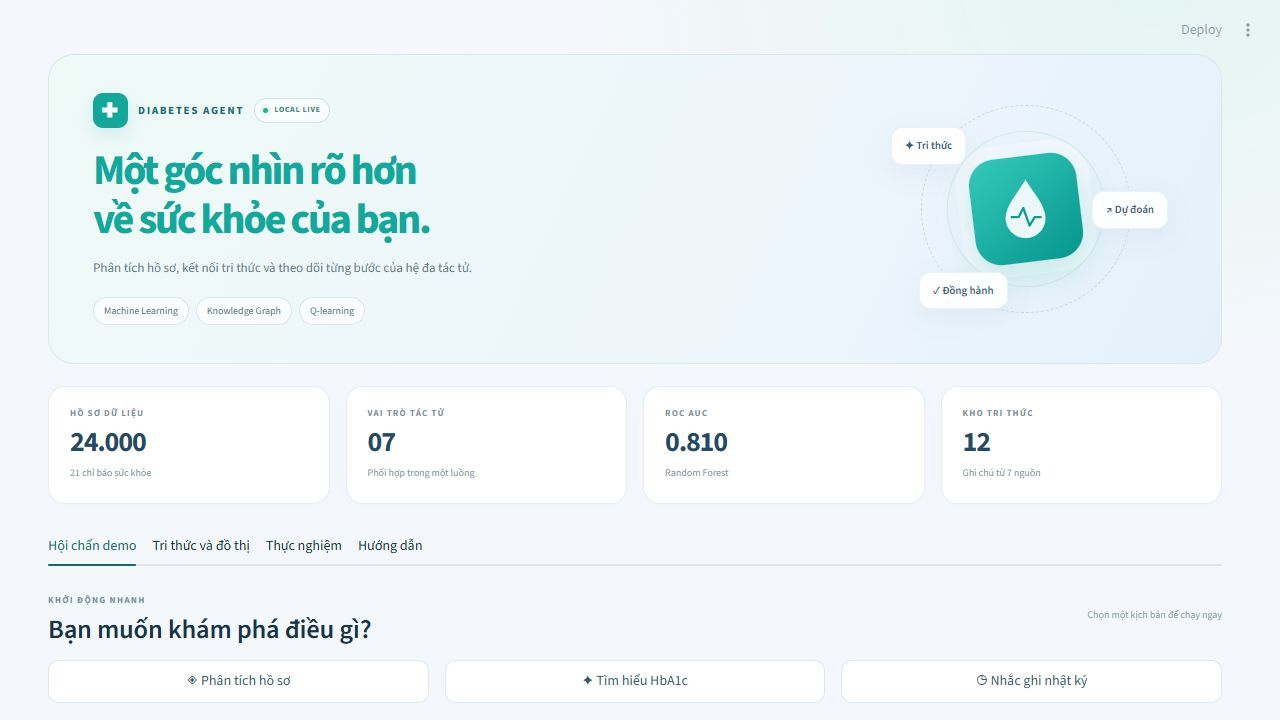
\includegraphics[width=\textwidth]{images/demo_overview.jpg}
\caption{Dashboard tổng quan và các nút chạy nhanh của Diabetes Agent.}\label{fig:demo_overview}
\end{figure}

\clearpage
\section{Kết quả phân loại và phối hợp tác tử}
Ở lượt hội chẩn trong Hình \ref{fig:demo_consult}, Random Forest trả score khoảng 0,147. Với ngưỡng 0,230 đã lưu trong artifact, kết quả thuộc lớp 0. Vòng điểm đi kèm tên mô hình và ngưỡng; các thẻ bên cạnh trình bày tri thức có nguồn và hành động nhắc nhật ký.

Luồng hoàn tất gồm Intake, ba nhánh chuyên môn, Council và Advisor, tạo 12 thông điệp request/response. Bảy thẻ trạng thái phía trên phản ánh các vai trò đã tham gia. Chi tiết phối hợp và nút tải JSON cung cấp proposal, evidence, trạng thái và thời gian xử lý của phiên.
\begin{figure}[H]\centering
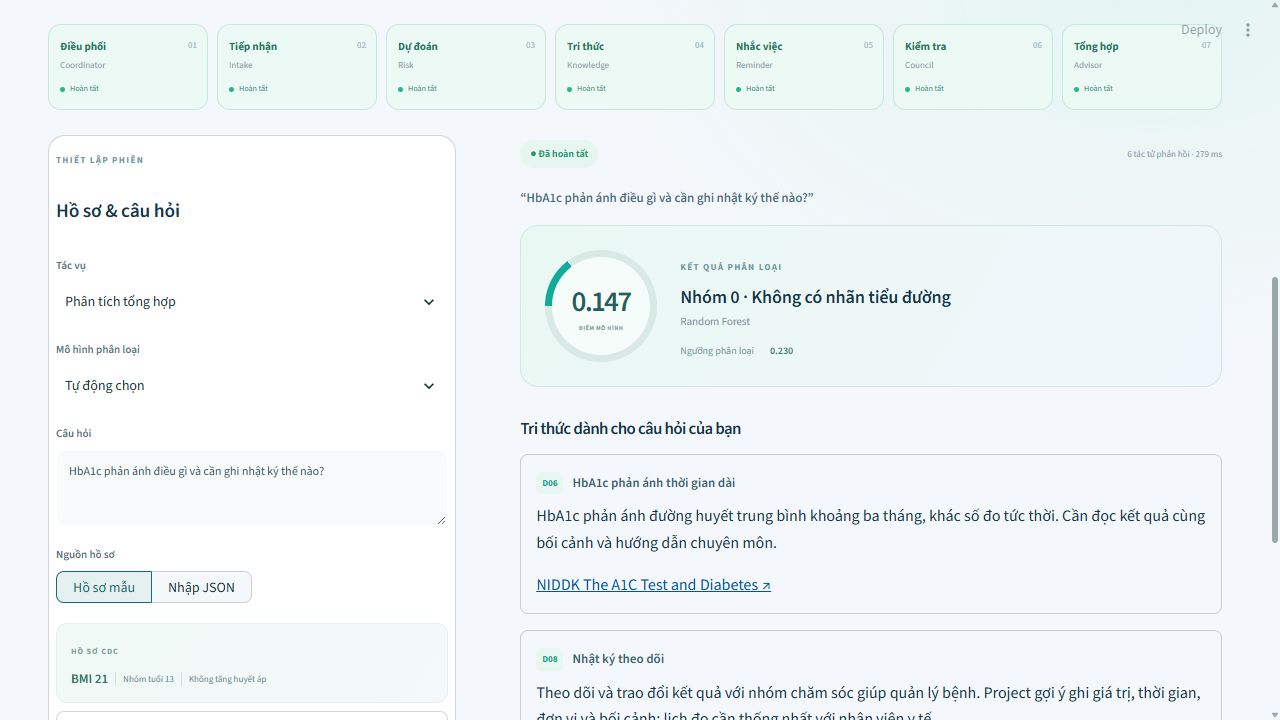
\includegraphics[width=\textwidth]{images/demo_consult.jpg}
\caption{Kết quả hội chẩn với score, ngưỡng phân loại và trạng thái tác tử.}\label{fig:demo_consult}
\end{figure}

\clearpage
\section{Tra cứu tri thức và bản đồ khái niệm}
Truy vấn \emph{HbA1c và thiếu máu} trả các ghi chú D07 và D06 trong ảnh chụp. Mỗi thẻ có ID, nội dung và liên kết nguồn. Bản đồ bên phải biểu diễn quan hệ giữa khái niệm xét nghiệm, HbA1c và các yếu tố ảnh hưởng đến kết quả xét nghiệm.

Tab này cho phép quan sát riêng nhánh Knowledge mà không chạy phân loại hồ sơ hoặc chính sách nhắc việc. Kết quả được lấy từ cùng bộ truy xuất dùng trong lượt hội chẩn.
\begin{figure}[H]\centering
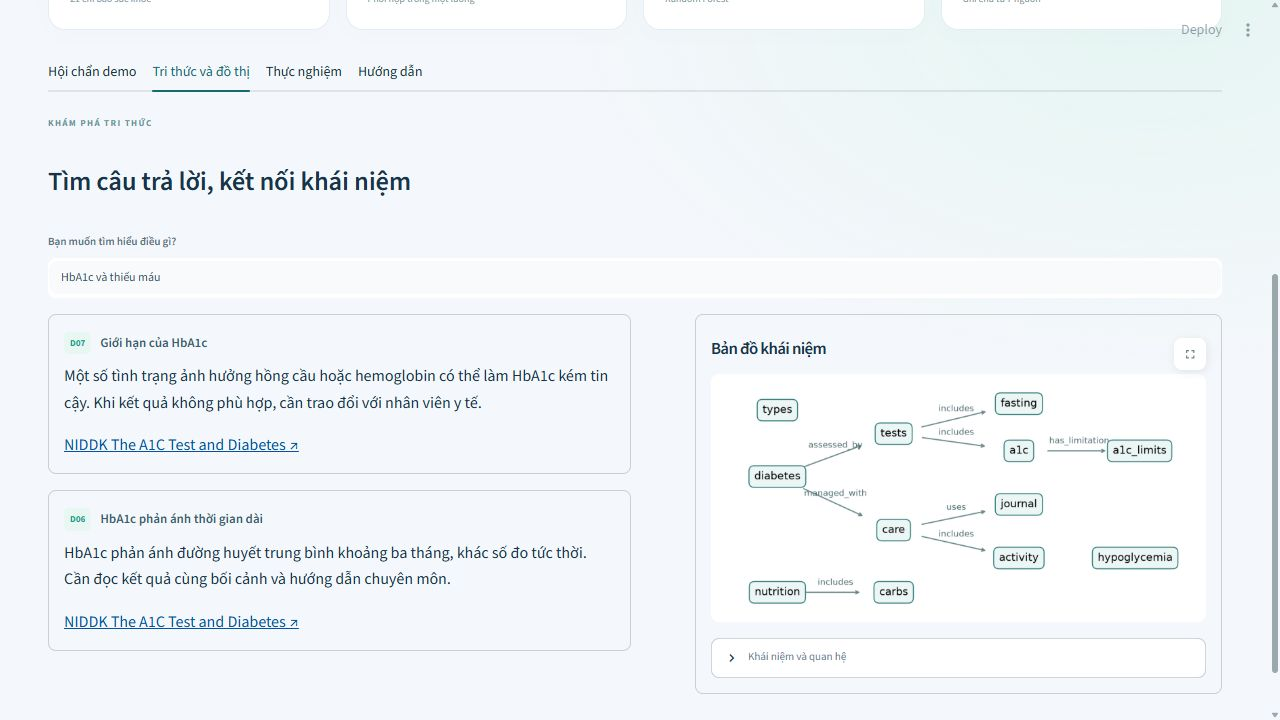
\includegraphics[width=\textwidth]{images/demo_knowledge.jpg}
\caption{Kết quả truy xuất theo câu hỏi và đồ thị khái niệm trên giao diện.}\label{fig:demo_knowledge}
\end{figure}

\clearpage
\section{Biểu đồ thực nghiệm trên giao diện}
Tab Thực nghiệm đọc các bảng đánh giá đã lưu. Bộ chọn chỉ số thay đổi biểu đồ giữa ROC AUC, Average Precision và F1. Với AP test, MLP đạt khoảng 0,3916; Random Forest đạt 0,3906; Logistic Regression đạt 0,3820; Dummy đạt 0,1373.

Biểu đồ nhắc việc hiển thị reward của các policy trong cùng simulator: fixed khoảng 0,2868, Q-learning 0,2703, rule 0,2006 và never 0,0876. Các đường cong và bảng chi tiết phía dưới sử dụng cùng artifact với phần thực nghiệm của báo cáo.
\begin{figure}[H]\centering
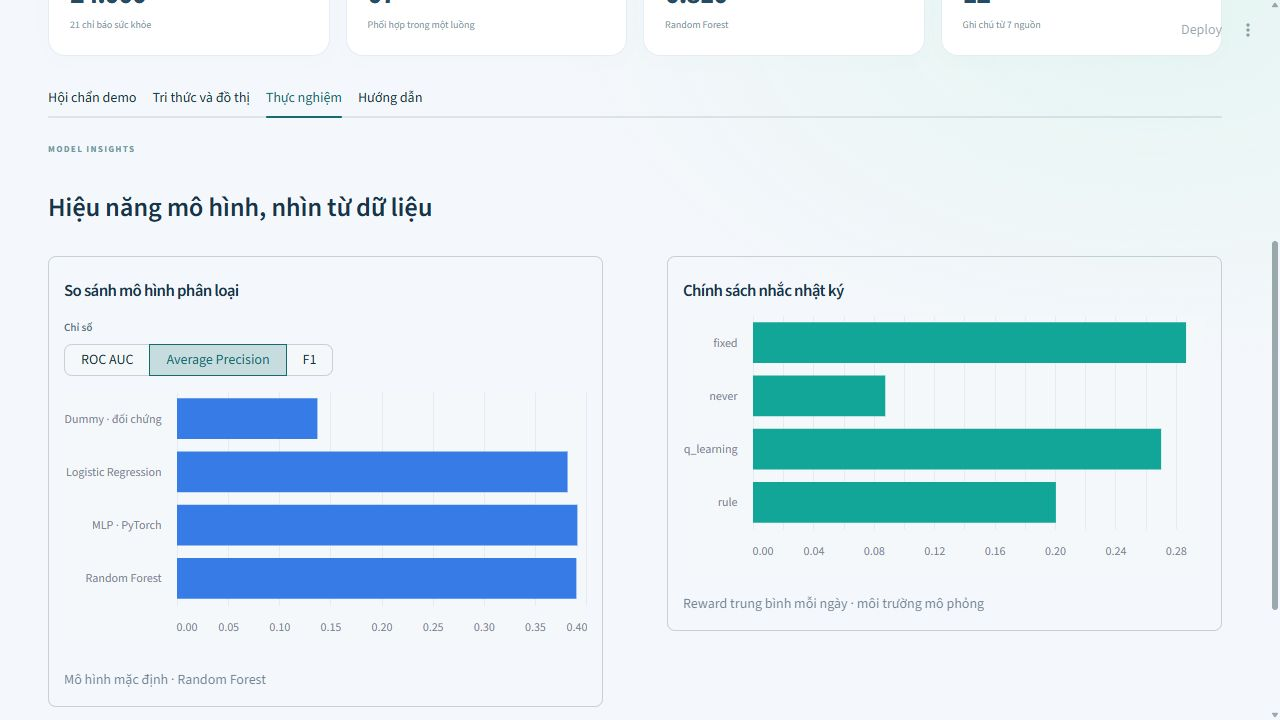
\includegraphics[width=\textwidth]{images/demo_benchmark.jpg}
\caption{Biểu đồ tương tác so sánh mô hình phân loại và chính sách nhắc việc.}\label{fig:demo_benchmark}
\end{figure}
